\newtheorem{theorem}{Teorema}[section]  % se ha reinicializado con la sección, si no se numeraría con ordinales continuos
\newtheorem{example}[theorem]{Ejercicio}
\newtheorem{definition}[theorem]{Definición}

\newcommand{\bom}{
\begin{tikzpicture}[line width=2pt,scale=0.2]
\draw (-1,0) .. controls (-2.5,3.5) and (2.5,3.5) .. (1,0);
\draw (-1,0) .. controls (0,-0.2) .. (1,0);
\draw (-1,0)--(-0.9,-0.2);\draw (1,0)--(0.9,-0.2);
\shade[shading=ball, ball color=yellow] (-1,0) .. controls (-2.5,3.5) and (2.5,3.5) .. (1,0);
\shade[shading=ball, ball color=yellow] (-1,0) .. controls (0,-0.2) .. (1,0);
\shade[shading=ball, ball color=yellow] (-1,0)--(-0.9,-0.2);\draw (1,0)--(0.9,-0.2);
\fill[color=gray] (-0.9,-0.2) .. controls (0,-0.4) .. (0.9,-0.2);
\draw (-0.9,-0.2)--(-0.8,-0.4);\draw (0.9,-0.2)--(0.8,-0.4);
\fill[color=gray] (-0.8,-0.4) .. controls (0,-0.6) .. (0.8,-0.4);
\draw (-0.8,-0.4)--(-0.7,-0.6);\draw (0.8,-0.4)--(0.7,-0.6);
\fill[color=gray] (-0.7,-0.6) .. controls (0,-0.8) .. (0.7,-0.6);
\draw (-0.7,-0.6)--(-0.5,-0.8);\draw (0.7,-0.6)--(0.5,-0.8);
\fill[color=black] (-0.5,-0.8) .. controls (0,-1) .. (0.5,-0.8);
\draw (-0.5,-0.8) .. controls (0,-1) .. (0.5,-0.8);
\draw (-0.3,-0.15)..controls (0,1.3) .. (-0.5,1.5);
\draw (0.3,-0.15)..controls (0,1.3) .. (0.5,1.5);
\draw (0.5,1.5)..controls (0,1.3) .. (-0.5,1.5);
\end{tikzpicture}}
\newcommand{\bomapa}{
\begin{tikzpicture}[line width=2pt,scale=0.2]
\draw (-1,0) .. controls (-2.5,3.5) and (2.5,3.5) .. (1,0);
\draw (-1,0) .. controls (0,-0.2) .. (1,0);
\draw (-1,0)--(-0.9,-0.2);\draw (1,0)--(0.9,-0.2);
\shade[shading=ball, ball color=gray] (-1,0) .. controls (-2.5,3.5) and (2.5,3.5) .. (1,0);
\shade[shading=ball, ball color=gray] (-1,0) .. controls (0,-0.2) .. (1,0);
\shade[shading=ball, ball color=gray] (-1,0)--(-0.9,-0.2);\draw (1,0)--(0.9,-0.2);
\fill[color=gray] (-0.9,-0.2) .. controls (0,-0.4) .. (0.9,-0.2);
\draw (-0.9,-0.2)--(-0.8,-0.4);\draw (0.9,-0.2)--(0.8,-0.4);
\fill[color=gray] (-0.8,-0.4) .. controls (0,-0.6) .. (0.8,-0.4);
\draw (-0.8,-0.4)--(-0.7,-0.6);\draw (0.8,-0.4)--(0.7,-0.6);
\fill[color=gray] (-0.7,-0.6) .. controls (0,-0.8) .. (0.7,-0.6);
\draw (-0.7,-0.6)--(-0.5,-0.8);\draw (0.7,-0.6)--(0.5,-0.8);
\fill[color=black] (-0.5,-0.8) .. controls (0,-1) .. (0.5,-0.8);
\draw (-0.5,-0.8) .. controls (0,-1) .. (0.5,-0.8);
\draw (-0.3,-0.15)..controls (0,1.3) .. (-0.5,1.5);
\draw (0.3,-0.15)..controls (0,1.3) .. (0.5,1.5);
\draw (0.5,1.5)..controls (0,1.3) .. (-0.5,1.5);
\end{tikzpicture}}



\section*{Introducción}
El algoritmo Advanced Encryption Standard, abreviado con las siglas AES, es el algoritmo más popular usado para protección elećtrónica de datos. Desde 2006 es el algoritmo más popular dentro de los algoritmos usados en lo que se llama \emph{criptografía simétrica}. La criptografía simétrica también es denominada criptografía de una clave, y es que la clave que se usa tanto para cifrar un mensaje como para descifrarlo es la misma. Así que receptor y emisor se ponen de acuerdo en esta misma clave.

Con este artículo se pretende dar un esquema sobre cómo funciona este tipo de algoritmos, qué matemática lo soporta y hacernos una idea de qué ocurre, por ejemplo,  cuando pasamos una tarjeta de prepago para el pago del billete del autobús, o como funcionan internamente las tarjetas prepago de energia como las que explicamos en la Seccion de Novedades de este numero.

En términos muy genéricos tenemos un emisor y un receptor. El emisor da una información (\textbf{input}) que es encriptada por el algoritmo que presentamos el receptor recibe esta información encriptada (\textbf{output}) y junto con la clave (\textbf{clave secreta}) que es conocida por ambos realiza el proceso de desencriptación. De este modo se ha transapasado una información con alta seguridad de que terceros no puedan tener acceso a ella. Veremos como es procesada esa información  en  el algoritmo, cómo procesa la clave y como realiza el proceso de encriptación, y en qué tipo de matemáticas está soportado todo este juego de encriptación. El proceso de desencriptación no lo veremos por ser bastante similar pero trabajando de forma inversa.

\section{Bytes y vector de bytes}

La unidad básica para procesar en el algoritmo AES es un {\textbf byte}: esto es una secuencia de ocho bits tratado como una unidad entera. Un bit es un dígito del sistema binario. En el sistema decimal que es el que usualmente se usa en la vida cotidiana, usamos 10 dígitos. En cambio para el sistema binario sólo se necesitan dos dígitos, el 0 y el 1. A nivel de placa informática, podemos imaginar el cero como apagado y el 1 como encendido. Véase un ejemplo de un byte de ocho bits representado  en la Figura \ref{fig:byte}.
\begin{figure}[!ht]
\begin{figurebox}
\begin{center}
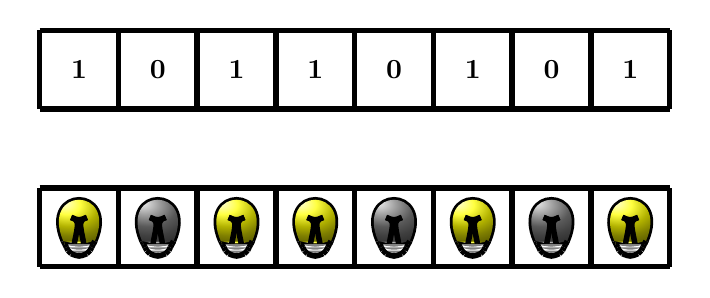
\begin{tikzpicture}[thick,line width=2pt]
\draw[step=1] (0,0) grid (8,1);
\node at (0.5,0.575) {\bom};
\node at (1.5,0.575) {\bomapa};
\node at (2.5,0.575) {\bom};
\node at (3.5,0.575) {\bom};
\node at (4.5,0.575) {\bomapa};
\node at (5.5,0.575) {\bom};
\node at (6.5,0.575) {\bomapa};
\node at (7.5,0.575) {\bom};
\draw[step=1] (0,2) grid (8,3);
\node at (0.5,2.5) {{\bf 1}};
\node at (1.5,2.5) {{\bf 0}};
\node at (2.5,2.5) {{\bf 1}};
\node at (3.5,2.5) {{\bf 1}};
\node at (4.5,2.5) {{\bf 0}};
\node at (5.5,2.5) {{\bf 1}};
\node at (6.5,2.5) {{\bf 0}};
\node at (7.5,2.5) {{\bf 1}};
\end{tikzpicture}
\end{center}\caption{Ejemplo de un byte de 8 bits en representación animada y binaria}\label{fig:byte}
\end{figurebox}
\end{figure}


 A partir de la unidad del byte podemos definir una lista de bytes o una matriz de bytes como se muestra en las Deficiones \ref{def1} y \ref{def2}.
\begin{definition}\label{def1}
Una lista de bytes es es una secuencia finita de $n\in \mathbb{N}$ bytes que podemos denotar como sigue,
$$a_0 a_1 ...a_{n-1}$$
donde $a_{i}$ es un byte para $i \in \{0,1,...,n-1\}$.
\end{definition}

\begin{definition}\label{def2}
Una matriz de bytes es un conjunto ordenado en filas y columnas cuyos elementos son bytes. Más particularmente diremos que $A$ es una matriz de $m$ filas y $n$ columnas y sus elementos se denotarán como  $a_{ij}$ para $i \in \{1,2,\dots, m\}$ y $j \in \{1,2,\dots, n\}$ siendo $a_{ij}$ un byte.
\end{definition}
Véase un ejemplo de una matriz cuadrada de tamaño $4$ en la Figura \ref{fig:matrizbytes}.

\begin{figure}
\begin{figurebox}
\begin{center}
$
\left[
\begin{array}{cccc}
a_{11} & a_{12} & a_{13} & a_{14}\\
a_{21} & a_{22} & a_{23} & a_{24}\\
a_{31} & a_{32} & a_{33} & a_{34}\\
a_{41} & a_{42} & a_{43} & a_{44}\\
\end{array}
\right]=\left[
\begin{array}{c|c|c|c}
10001001 & 11110000 & 10101010 & 10010011\\\hline
10011111 & 10010100 & 01001001 & 10111111\\\hline
00001001 & 01010101 & 10101011 & 10011001\\\hline
01011101 & 10010011 & 10110001 & 01011101\\
\end{array}
\right]
$
\end{center}\caption{Ejemplo de una matriz de bytes}\label{fig:matrizbytes}
\end{figurebox}
\end{figure}



\subsection{Entradas(input), salidas(output) y clave secreta}\label{ss:input}

La entrada y la salida para el algoritmo AES consiste en un array de 16 bytes, esto hace un total de 128 bits. En el proceso interno del algoritmo estos 128 bits serán operados como una matriz de bytes de 4 por 4 como hemos visto en la Figura \ref{fig:matrizbytes}. De esta manera el input o entrada del algoritmo es representado como el siguiente array  $in_{0}in_{1}...\,in_{15}$  y el output o salida como $out_{0}out_{1}...\,out_{15}$ donde cada $in_{i}$ y  $out_{i}$ es un byte para $i \in \{0,1,...,15\}$. Internamente, la entrada y todas las modificaciones, que denominamos {\textsl estados intermedios},  que producirá el algoritmo serán trabajados como matrices de bytes de tamaño $4$ por $4$ como puede verse en la Figura \ref{fig:inout}.

\begin{figure}[!ht]
\begin{figurebox}
\begin{center}
\tiny{$ \underbrace{in_{0}in_{1}...\,in_{15}}_{\text{entrada}} \rightarrow
\left[
\begin{array}{cccc}
in_{0} & in_{4} & in_{8} & in_{12}\\
in_{1} & in_{5} & in_{9} & in_{13}\\
in_{2} & in_{6} & in_{10} & in_{14}\\
in_{3} & in_{7} & in_{11} & in_{15}\\
\end{array}
\right] \rightarrow \underbrace{\left[
\begin{array}{cccc}
s_{00} & s_{01} & s_{02} & s_{03}\\
s_{10} & s_{11} & s_{12} & s_{13}\\
s_{20} & s_{21} & s_{22} & s_{23}\\
s_{30} & s_{31} & s_{32} & s_{33}\\
\end{array}
\right]}_{\text{estados intermedios}} \rightarrow \left[
\begin{array}{cccc}
out_{0} & out_{4} & out_{8} & out_{12}\\
out_{1} & out_{5} & out_{9} & out_{13}\\
out_{2} & out_{6} & out_{10} & out_{14}\\
out_{3} & out_{7} & out_{11} & out_{15}\\
\end{array}
\right] \rightarrow  \underbrace{out_{0}out_{1}...\,out_{15}}_{\text{salida}}
$
}
\end{center}\caption{Entrada, salida y estados intermedios.}\label{fig:inout}
\end{figurebox}
\end{figure}

En el algoritmo los estados intermedios pueden verse desde otro punto de vista. Los cuatro bytes que forman cada columna dan un total de 32 bits. Así que el estado puede ser interpretado como un vector columna  de cuatro palabras cada una de ellas formada con 32 bits. Así, por ejemplo,  el estado intermedio representado en la Figura \ref{fig:inout} puede ser considerado como un vector columna de las siguientes palabras:
$$
w_0=s_{00}s_{10}s_{20}s_{30}, \quad w_1=s_{01}s_{11}s_{21}s_{31}, \quad, w_2=s_{02}s_{12}s_{22}s_{32}, \quad w_3=s_{03}s_{13}s_{23}s_{33}.
$$

La clave secreta también es un array de bytes, pero tenemos tres posibilidades: 16 bytes(128 bits), 24 bytes(192 bits) o 32 bytes(256 bits). En el caso de 128 bits la clave inicial y las posteriores procesadas en el algoritmo serán procesadas como bloques de tamaño 4 por 4; en el caso de 192 bits bloques de tamaño 4 por 6 y finalmente en el caso de 256 bites bloques de tamaño 4 por 8.


\subsection{Interpretaciones distintas de un byte}

Parece divertido que un byte de ocho bits puede ser interpretado como un polinomio o como una pareja de elementos hexadecimales. Vamos a ver de qué se trata esto.

\begin{center}
\textbf{Notación polinomial}
\end{center}

Representamos un byte de ocho dígitos como sigue $\{b_7, b_6,b_5,b_4,b_3,b_2,b_1,b_0\}$. Este byte puede ser representado como un polinomio $p(x)$ de grado siete como sigue:
\begin{equation}\label{eq:pol}
p(x)=b_7 x^7 +b_6 x^6+b_5 x^5+b_4 x^4+b_3 x^3+b_2 x^2+b_1 x+b_0=\sum_{k=0}^7 b_k x^k.
\end{equation}

Por ejemplo, el byte $\{01101011\}$ representa el polinomio $x^6+x^5+x^3+x+1$.

\begin{center}
\textbf{Notación hexadecimal}
\end{center}

El sistema hexadecimal consta de 16 digitos: 0,1,2,3,4,5,6,7,8,9,A,B,C,D,E,F. La letra $A$ representa el 10, la letra $B$ el once y así sucesivamente. Por ejemplo, el número 143 en notación decimal se corresponde con $10011110$ en notación binaria y con $9E$ con notación hexadecimal. La representación hexadecimal que vamos a hacer de un byte se realiza mediante la siguiente representación:
\begin{center}
\begin{tabular}{|c|c||c|c||c|c||c|c|}\hline
Patrón & Carácter & Patrón & Carácter & Patrón & Carácter & Patrón & Carácter\\\hline
0000 & 0 & 0100 & 4 & 1000 & 8 & 1100 & C\\
0001 & 1 & 0101 & 5 & 1001 & 9 & 1101 & D\\
0010 & 2 & 0110 & 6 & 1010 & A & 1110 & E\\
0011 & 3 & 0111 & 7 & 1011 & B & 1111 & F\\\hline
\end{tabular}
\end{center}
Usando este patrón si tomamos, por ejemplo,  el byte $\{10011110\}$ se correponde en notación hezadecimal con los primeros cuatro dígitos se corresponde con el 9 en notación hexadecimal y los últimos cuatro dígitos con el E. Esto es se corresponde con el par $9E$. Usando este patrón podemos representar la matriz dada en la Figura \ref{fig:matrizbytes} en notación hexadecimal como sigue:
$$\left[
\begin{array}{c|c|c|c}
89 & F0 & AA & 93\\\hline
9F & 94 & 49 & BF\\\hline
09 & 54 & AB & 99\\\hline
5D & 93 & B1 & 5D\\
\end{array}
\right].$$


\section{Las matemáticas del algoritmo}
Todos los bytes en el algoritmo AES son interpretados como polinomios de grado 7 con coeficientes $0$ o $1$. Desde un punto de vista más matemático y propio diríamos que los bytes están interpretados como elementos del campo finito $\mathcal{GF}$($2^8$) (véase \cite{Hart}). No vamos a entrar en detalles y vamos a hablar de la manera más sencilla, pero si desea saber más de lo que es un cuerpo finito, los polinomios, las estructuras algebraicas, remitase a las referencias siguientes \cite{Hart,Hilton,HUnger} , ¡es un mundo amazónico!

Vamos a ver qué operaciones podemos hacer entre los bytes mediante la representación polinomial descrita en la Ecuación (\ref{eq:pol}).
\subsection{Suma}\label{ss:suma}
Sean dos bytes $a=\{a_7,a_6,a_5,a_4,a_3,a_2,a_1,a_0\}$ y $b=\{b_7,b_6,b_5,b_4,b_3,b_2,b_1,b_0\}$, definimos la suma $c=\{c_7,c_6,c_5,c_4,c_3,c_2,c_1,c_0\}$ entre $a$ y $b$ y que denotamos como $a \oplus b$ como sigue:
\begin{description}
\item[Notación de byte:]
$c=a\oplus b=\{c_7,c_6,c_5,c_4,c_3,c_2,c_1,c_0\}=\{a_7 \oplus b_7,a_6 \oplus b_6,a_5 \oplus b_5,a_4 \oplus b_4,a_3 \oplus b_3,a_2 \oplus b_2,a_1\oplus b_1 ,a_0 \oplus b_0\}$ donde $\oplus$ denota la operación XOR binaria, esto es: $0 \oplus 0=0, 1 \oplus 0=0 \oplus 1=1, 1 \oplus 1=0 $.
\item[Notación polinomial:] $\sum_{k=0}^7 c_k x^k=\sum_{k=0}^7 (a_k \oplus b_k) x^k$, siendo $\oplus$ la operación definida en el anterior item.
\end{description}
\begin{example}
La suma del polinomio $x^7+x^6+x^4+x+1$ con $x^7+x^4+x+1$ nos da como resultado el polinomio $x^6$ que se corresponde con el byte $\{01000000\}$.
\end{example}

\subsection{Multiplicación}\label{ss:prod}
La multiplicación que vamos a explicar no es tan intuitiva como la suma anterior. De hecho vamos a hacer una parada para hablar de la operación {\sl módulo}.

Fijémonos en esto: cuando dividimos cualquier número natural por 2, tenemos dos opciones de resto, el 0 y el 1. Esta distinción no es otra que hablar de números pares e impares. Más formalmente, sean  todos los números enteros $\mathbb{Z}$ y realicemos la división entre dos. Tenemos una colección de números cuyo resto es 0, y otros cuyo resto es 1. Desde este punto de vista podemos hablar de $\mathbb{Z}_2$ (espacio cociente) que es un cuerpo con dos únicos elementos: la clase de los elementos pares y la clase de los elementos impares. Fíjate que la operacion XOR binaria definida antes tiene mucha relación con esto. De hecho entender la operacion $1 \oplus 1= 0$ es muy simple ahora si piensas que {\sl la suma de dos números impares es un número par}.

Podemos pensar en hacer algo similar por ejemplo dividiendo por 5. De esta manera el conjunto de números enteros podría ser descompuesto en 5 clases: los divisibles por 5 (clase [0]), los que dan resto 1 (clase [1]), los que dan resto 2 (clase [2]) , los que dan resto 3 (clase [3]) y los que dan resto 4 (clase [4]). ¿En qué clase se encuentra el número 1234?

¿Te parece la operación modular extraña? ¿Te imaginas que podemos hacer lo mismo con polinomios? Pues también se puede. Imaginemos el polinomio \mbox{$x^{13}+ x^{11}+x^9+x^8+ x^6+x^5+x^4+x^3+1$} y dividámoslo por el polinomio irreducible de grado ocho : \mbox{$x^8+x^4+x^3+x+1$}. Si dividimos ambos polinomios (hazlo como ejercicio para recordar como dividir dos polinomios) el resto que queda es el polinomio : \mbox{$x^7+x^6+1$}. De manera más genérica: si tenemos un polinomio $p(x)$ y otro polinomio de menor o igual grado $q(x)$, diremos que $r(x)$ es $p(x)$ módulo $q(x)$ siendo $r(x)$ el resto de dividir $p(x)$ entre $q(x)$.

Dado este supuesto salto o paréntesis, vamos a entender el por qué de todo esto. Como se titula esta subsección es multiplicación, esto es multiplicación de dos polinomios que cada uno de ellos representa un byte. Pero si recuerdas como multiplicar dos polinomios el grado del polinomio producto es la suma de los grados de los polinomios. Por ejemplo, si multiplicas un polinomio de grado 3 por otro de grado 6 el resultado será un polinomio de grado 9. Pero en todo momento hemos dicho que el algoritmo AES trabajará com polinomios de grado menor o igual que 7. Entonces si multiplicamos polinomios de grado a lo sumo siete tendremos en la mayoría de los casos polimonios de grado mayor que siete. Esta  la razón por la que la multiplicación no es la usual si no que la multiplicación que se define es la usual seguida de  una operación modular con el polinomio irreducible siguiente:
\begin{equation}\label{eq:q}
q(x)=x^8+x^4+x^3+x+1.
\end{equation} Al ser $q(x)$ un polinomio de grado $8$ siempre el resto tendrá un grado a lo sumo $7$, obteniendo lo que queríamos, trabajar con bytes. Esta multiplicación la denotaremos como $a(x) \bullet b(x)$ o en notación de bytes como $a\bullet b$ entre $a$ y $b$.
\begin{example}
Sean los polinomios $a(x)=x^6+x^4+x^2+x+1$ y $b(x)=x^7+x+1$, su multiplicación usual  es \mbox{$x^{13}+ x^{11}+x^9+x^8+ x^6+x^5+x^4+x^3+1$} y operación modular con $q(x)$ dado en la Ecuación (\ref{eq:q}) da como resultado el polinomio  \mbox{$x^7+x^6+1$}. Así,
$$
a(x)\bullet b(x)=x^7+x^6+1.
$$
\end{example}
Observemos que en la operación de multiplicar los polinomios se da la multiplicación entre elementos binarios, esto es: $1 \cdot 1=1, 1 \cdot 0= 0\cdot 1= 0, 0 \cdot 0 =0$.


%\subsection{Multiplicación por x}
%De nuevo, si tenemos un polinomio de a lo sumo grado siete si multiplicamos por $x$ este será a lo sumo de grado ocho, por lo que dejaríamos de %trabajar con polinomios de grado menor o igual que siete, es por ello que de nuevo hablamos de multiplicación realizando módulo el polinomio %$q(x)$ definido en la ecuación (\ref{eq:q}). Veamos que hacer esto da como resultado una operación curiosa. Veámoslo primero con unos ejemplos.

%Sea $z(x)=x^6+x^2+x+1$, entonces el polinomio $x \cdot z(x)= x^7+x^3+x^2+x$ y módulo $q(x)$ coincide con el mismo por ser de menor grado que %ocho. Tomemos otro ejemplo donde el coeficiente del monomio de grado 7 no es cero. Sea $s(x)=x^7+x^5+x^2+x+1$, entonces el polinomio $x \cdot %s(x)= x^8+x^6+x^3+x^2+x$ y si realicemos la división con el polinomio $q(x)$ dado en la Ecuación (\ref{eq:q}) tenemos que el resto es el %polinomio resultanter de realizar la operación $x \cdot s(x)-q(x)$. De esta maenra el resultado final es el polinomio $x^6+x^4+x^2+1$. Si %miramos esto con bytes, la operación de multiplicar por $x$ cuando $b_7 \neq 0$ (mire la notación expuesta en la ecuación (\ref{eq:pol})) es %equivalente ha crear un byte corriendo los digitos a la izquierda y realizar la operación XOR con el byte $(1b)=\{00011011\}$. Así el polinomio  %$s(x)$ del ejemplo anterior que se corresponde con el byte $(A7)=\{10100111\}$, le hacemos un movimiento a la izquierda y nos da  $\{01001111\}$ %y sumamos con $(1b)=\{00011011\}$, obteniendo el byte $(\{01010100\}$ que se corresponde con $x^6+x^4+x^2+1$. Esta operación es la que el %algoritmo AES ha denominado {\sl xtime()}. La repetición de esta operación permite la multiplicación de potencias de $x$.

\subsection{Polinomios con coeficientes que son bytes de ocho dígitos}

En la subsección \ref{ss:input} hablamos de palabras como unos vectores columnas de 32 bits concatenados. Vamos a ver como trabajar con todo esto y que matemática modeliza esto. Antes hemos hablado de polinomios de grado menor o igual que siete con coeficientes en $\mathbb{Z}_2$, es to es o 0 o 1. Ahora vamos a definir el siguiente polinomio.
\begin{equation}\label{def:polwo}
a(x)=a_3 x^3+a_2 x^2+ a_1 x + a_0,
\end{equation}
donde $a_3,a_2,a_1$ y $a_0$ son bytes de ocho dígitos. Vamos a ver como hemos hecho en las anteriores subsecciones, con este tipo de polinomios como son las operaciones suma y multiplicación entre dos polinomios dados como la ecuación (\ref{def:polwo}).
\subsubsection{Suma}\label{ss:sumarara}
Esta es muy intuitiva,  pues basta sumar los bytes como vimos en la subsección \ref{ss:suma}. De este modo sean $a(x)=a_3 x^3+a_2 x^2+ a_1 x + a_0$ y $b(x)=b_3 x^3+b_2 x^2+ b_1 x + b_0$ dos polinomios como en la ecuación (\ref{def:polwo}), entonces la suma denotada como $a(x)+b(x)$ será la siguiente:
$$
a(x)+b(x)=(a_3 \oplus b_3) x^3+(a_2 \oplus b_2) x^2+ (a_1 \oplus b_1) x + (a_0 \oplus b_0).
$$
\begin{example}
Sea $a(x)=\{10000001\} x^3+\{11100001\} x^2+ \{10101010\} x +\{01010100\}$ y $b(x)=\{10000001\} x^3+\{00000001\} x^2+ \{10101010\} x +\{00000000\}$ polinomios con coeficientes bytes, es fácil chequear que
$$
a(x)+b(x)=\{00000000\} x^3+\{11100000\} x^2+ \{00000000\} x +\{01010100\}.
$$
\end{example}
\subsubsection{Multiplicación}\label{ss:prodraro}
Esta operación sigue un razonamiento similar al realizado en la subsección \ref{ss:prod}. Pero es algo más complicado.
\begin{description}
\item[Paso multiplicativo] Creamos el polinomio producto $c(x)$ a partir de $a(x)$ y $b(x)$ dados como antes, como sigue:
$$
c(x)=c_6x^6+c_5x^5+c_4 x^4+c_3 x^3 +c_2 x^2 +c_1 x+c_0,
$$
donde
\begin{equation}\label{eq:progf}
\begin{array}{ll}
c_0= a_0 \bullet b_0, & c_1=a_1\bullet b_0 \oplus a_0 \bullet b_1,\\
c_2=a_2\bullet b_0 \oplus a_1 \bullet b_1 \oplus a_0 \bullet b_2 , & c_3= a_3\bullet b_0 \oplus a_2 \bullet b_1 \oplus a_1 \bullet b_2 \oplus a_0\bullet b_3,\\
c_4=a_3\bullet b_1 \oplus a_2 \bullet b_2 \oplus a_1 \bullet b_3, &  c_5=a_3\bullet b_2 \oplus a_2 \bullet b_3,\\
c_6=a_3\bullet b_3. & \\
\end{array}
\end{equation}
\item[Paso modular] Como el resultado en la ecuación (\ref{eq:progf}) no es un polinomio de cuatro palabras tenemos que realizar una operación modular con un polinomio de grado 4. El algoritmo AES lo realiza con el polinomio $x^4+1$. Esta operación te la dejamos como ejercicio para que practiques (puedes ver todo los detalles en \cite{Federal}).
\end{description}

Finalmente si trabajas lo que te hemos propuesto se puede ver que realizar el producto entre $a(x)$ y $b(x)$ el cual denotaremos como $a(x)\otimes b(x)$ es equivalente a realizar una operación matricial donde las sumas y productos son los explicados en la subsección anterior, esto es $\bullet$ y $\oplus$ entre bytes. Así \mbox{$a(x)\otimes b(x)=d(x)=d_3x^3+d_2 x^2+d_1 x+d_0$} donde
$$
\left[
\begin{array}{c}
d_0\\
d_1\\
d_2\\
d_3\\
\end{array}
\right]=\left[
\begin{array}{cccc}
a_0 & a_3 & a_2 & a_1\\
a_1 & a_0 & a_3 & a_2\\
a_2 & a_1 & a_0 & a_3\\
a_3 & a_2 & a_1 & a_2\\
\end{array}
\right]\left[
\begin{array}{c}
b_0\\
b_1\\
b_2\\
b_3\\
\end{array}
\right]
$$
Observemos que si tomamos como polinomio $a(x)=\{00000001\}x^3$ el resultado del producto de $a(x)\otimes b(x)$ es una rotación de la palabra $[b_0, b_1,b_2,b_3]$; esto es $[b_1, b_2,b_3,b_0]$. Esta operación la denotará el algoritmo AES como {\textsl rotWord()}.
\section{Un esquema del algoritmo}

Antes de dar las ideas del algoritmo queremos remarcar varios puntos:
\begin{itemize}
\item La longitud de la entrada y salida es de 128 bits representados en bloques de tamaño cuatro por cuatro, cada elemento un byte (usando notación hexadecimal nos será más fácil representarlo).
\item La longitud de la clave secreta dependerá de que tipo de algoritmo AES use. Se distinguen tres AES-128, AES-192 y AES-256, los cuales usan una clave secreta, respectivamente de 128 bits, 192 bits y 256 bits.
\item El número de vueltas que se dará al algoritmo dependerá  también de que tipo de AES. El AES.128 realizará 10 vueltas, el AES-192 doce y el AES-256 realizará 14.
\end{itemize}

Para no complicar demasiado el algorimo solo veremos el proceso de encriptación. El proceso de desencriptación es similar pero con operaciones invesas.
\subsection{Input del algoritmo}

El estado y la clave secreta. Usando notación hexadecimal tendríamos algo así:
\begin{figure}[!ht]
\begin{figurebox}
\begin{center}
$\begin{array}{|c|c|c|c|}
\multicolumn{4}{c}{\text{ESTADO INICIAL}}\\\hline
04 & E0 & 48 & 28\\\hline
66 & CB & F8 & 06\\\hline
81 & 19 & D3 & 26\\\hline
E5 & 9A & 7A & 4C\\\hline
\end{array}
\quad
\begin{array}{|c|c|c|c|}
\multicolumn{4}{c}{\text{CLAVE SECRETA}}\\\hline
A0 & 88 & 23 & 2A\\\hline
FA & 54 & A3 & 6C\\\hline
FE & 2C & 39 & 76\\\hline
17 & B1 & 39 & 05\\\hline
\end{array}
$
\end{center}\caption{Input del Algoritmo AES-128}\label{fig:inputaes1}
\end{figurebox}
\end{figure}

\subsection{Proceso de encriptación del estado}
Distinguimos tres etapas:
\begin{center}{\bf Ronda inicial}\end{center}
\begin{figure}[!ht]
\begin{figurebox}
\begin{center}
$\begin{array}{|c|c|c|c|}
\multicolumn{4}{c}{\text{ESTADO INICIAL}}\\\hline
04 & E0 & 48 & 28\\\hline
66 & CB & F8 & 06\\\hline
81 & 19 & D3 & 26\\\hline
E5 & 9A & 7A & 4C\\\hline
\end{array},
\begin{array}{|c|c|c|c|}
\multicolumn{4}{c}{\text{CLAVE SECRETA}}\\\hline
A0 & 88 & 23 & 2A\\\hline
FA & 54 & A3 & 6C\\\hline
FE & 2C & 39 & 76\\\hline
17 & B1 & 39 & 05\\\hline
\end{array}\rightarrow
\colorbox{pink}{AddRoundKey}\rightarrow \begin{array}{|c|c|c|c|}
\multicolumn{4}{c}{\text{ESTADO 0}}\\\hline
A4 & G8 & 6B & 02\\\hline
9C & 9F & 5B & 6A\\\hline
7F & 35 & EA & 50\\\hline
F2 & 2B & 43 & 49\\\hline
\end{array}
$
\end{center}\caption{Ronda Inicial del algoritmo AES-128}\label{fig:inputaes1}
\end{figurebox}
\end{figure}


\begin{center}{\bf 9 rondas}\end{center}
\begin{figure}[!ht]
\begin{figurebox}
\begin{center}
$\begin{array}{|c|c|c|c|}
\multicolumn{4}{c}{\text{ESTADO $(i-1)$ésimo}}\\\hline
A4 & G8 & 6B & 02\\\hline
9C & 9F & 5B & 6A\\\hline
7F & 35 & EA & 50\\\hline
F2 & 2B & 43 & 49\\\hline
\end{array}\rightarrow$
\begin{tabular}{l}
\\
\colorbox{green}{1. SubBytes}\\
\colorbox{yellow}{2. ShiftRows}\\
\colorbox{gray}{3. Mixcolums } \\
\colorbox{pink}{4. AddRoundKey} con
\tiny{
$\begin{array}{|c|c|c|c|}
\multicolumn{4}{c}{\text{CLAVE $(i)$-ésima}}\\\hline
* & * & * & *\\\hline
* & * & * & *\\\hline
* & * & * & *\\\hline
* & * & * & *\\\hline
\end{array}$
}
\\
\end{tabular} $\rightarrow
\begin{array}{|c|c|c|c|}
\multicolumn{4}{c}{\text{ESTADO i+1-ésimo}}\\\hline
A4 & G8 & 6B & 02\\\hline
9C & 9F & 5B & 6A\\\hline
7F & 35 & EA & 50\\\hline
F2 & 2B & 43 & 49\\\hline
\end{array}
$
\end{center}\caption{Ronda i-ésima del algoritmo AES-128 para $i\in\{1,2,...,9\}$}\label{fig:inputaes2}
\end{figurebox}
\end{figure}

\begin{center}{\bf Ronda final}\end{center}
\begin{figure}[!ht]
\begin{figurebox}
\begin{center}
$\begin{array}{|c|c|c|c|}
\multicolumn{4}{c}{\text{ESTADO 9}}\\\hline
E9 & CB & 3D & AF\\\hline
09 & 31 & 32 & 2E\\\hline
89 & 07 & 7D & 2C\\\hline
72 & 5F & 94 & B5\\\hline
\end{array}\rightarrow$
\begin{tabular}{l}
\\
\colorbox{green}{1. SubBytes}\\
\colorbox{yellow}{2. ShiftRows}\\
\colorbox{pink}{3. AddRoundKey} con
\tiny{
$\begin{array}{|c|c|c|c|}
\multicolumn{4}{c}{\text{CLAVE  9-ésima}}\\\hline
* & * & * & *\\\hline
* & * & * & *\\\hline
* & * & * & *\\\hline
* & * & * & *\\\hline
\end{array}$
}
\\
\end{tabular} $\rightarrow
\begin{array}{|c|c|c|c|}
\multicolumn{4}{c}{\text{ESTADO FINAL}}\\\hline
39 & 02 & DC & 19\\\hline
25 & DC & 11 & 6A\\\hline
84 & 09 & 85 & 0B\\\hline
1D & FB & 57 & 32\\\hline
\end{array}
$
\end{center}\caption{Última ronda del algoritmo AES-128}\label{fig:inputaes3}
\end{figurebox}
\end{figure}

%\newpage

En las Figuras \ref{fig:inputaes1}, \ref{fig:inputaes2} y \ref{fig:inputaes3} se muestra un esquema del proceso de encriptación del algoritmo AES  y en la. El proceso de desencriptación es bastante análogo pero con operaciones inversas. En la sección anexo pondremos claros ejemplos de lo que hacen cada una de las operaciones que aparecen en el esquema, estas son: SubBytes(), ShiftRows(), MixColumns(), AddRoundKey().

\subsection{Proceso de clave}
La clave inicial irá modificándose a lo largo del proceso para ser utilizada del modo que se presenta en las figuras \ref{fig:inputaes2} y \ref{fig:inputaes3}. Este proceso consiste en dada la clave inicial la cual la veremos como un array de cuatro palabras, cada palabra serán los 32 bits que encontramos en cada columna. Para generar la primera palabra de la clave ronda 1, lo que se hara es aplicar a la palabra 4 de la actual clave la operacion {\sl RotWord()} que vimos en la subsección \ref{ss:prodraro} y una vez hecho esto se le sumará la primera palabra y la primera columna de la matriz Rcon que aparece en la tabla \ref{tab:Rcon}. La segunda palabra se calcula a partir de la calculada sumando la segunda de la clave anterior; idem con la tercera y la cuarta. Y esta seria la clave ronda 1. Las nueve restantes se calculan de manera analoga siempre usando la anterior.

\begin{table}[ht!]
\begin{center}
$RCON=$\tiny{$\left[
\begin{array}{cccccccccc}
 01 & 02 & 04 & 08 & 10 & 20 & 40 & 80 & 1B & 36\\
 00 & 00 & 00 & 00 & 00 & 00 & 00 & 00 & 00 & 00\\
 00 & 00 & 00 & 00 & 00 & 00 & 00 & 00 & 00 & 00\\
 00 & 00 & 00 & 00 & 00 & 00 & 00 & 00 & 00 & 00\\
\end{array}\right]$}
\end{center}\caption{Matriz Rcon, cada columna representa la potencia $x^i$ modulo $q(x)$ para $i\in\{0,1,2,\dots, 9\}$.}\label{tab:Rcon}
\end{table}


\section{Conclusiones}

El proceso de desencriptación es muy similar a lo mostrado pero las operaciones que se utilizan y que se explican en el Anexo \ref{Anexo} deben verse de manera inversa. Todos los detalles puedes verlo en \cite{Federal}. Si deseas ver ejemplos puedes remitirte a \cite{Java} donde aparece un programa y códigos de las partes de los algoritmos.

\newpage

\section*{Anexo: las operaciones del proceso de encriptación}\label{Anexo}
Aquí vamos a representar de manera informal y con simples ejemplos cada una de las operaciones que aparecen en el proceso de encriptación del Algoritmo RSA-128 . Por simplicidad trabajaremos con notación hexadecimal.
\begin{enumerate}
\item {\bf SubBytes(\cdot)}: es una transformación no lineal que sustitute cada byte de un estado por otro usando una tabla de sustitución. Esta tabla se denomina S-box (véase \cite{Federal} para ver el origen de esta).
\begin{table}[ht!]
\begin{center}
\tiny{
\begin{tabular}{|c|c|c|c|c|c|c|c|c|c|c|c|c|c|c|c|c|c|}\hline
& & \multicolumn{16}{c|}{$y$}\\\hline
& &{\textbf 0} & {\textbf 1} & {\textbf 2} & {\textbf 3} & {\textbf 4} & {\textbf 5} & {\textbf 6} & {\textbf 7} & {\textbf 8} & {\textbf 9} & {\textbf A} & {\textbf B} & {\textbf C} & {\textbf D} & {\textbf E} & {\textbf F}\\
\multirow{16}{*}{$x$} & {\textbf 0} & 63 & 7C & 77 & 7B & F2 & 6B & 6F & C5 & 30 & 01 & 67 & 2B & FE & D7 & AB & 76 \\
                    & {\textbf 1} & CA & 82 & C9 & 7D & FA & 59 & 47 & F0 & AD & D4 & A2 & AF & 9C & A4 & 72 & C0 \\
                    & {\textbf 2} & B7 & FD & 93 & 26 & 36 & 3F & F7 & CC & 34 & A5 & E5 & F1 & 71 & D8 & 31 & 15 \\
                    & {\textbf 3} & 04 & C7 & 23 & C3 & 18 & 96 & 05 & 9A & 07 & 12 & 80 & E2 & EB & 27 & B2 & 75 \\
                    & {\textbf 4} & 09 & 83 & 2C & 1A & 1B & 6E & 5A & A0 & 52 & 3B & D6 & B3 & 29 & E3 & 2F & 84 \\
                    & {\textbf 5} & 53 & D1 & 00 & ED & 20 & FC & B1 & 5B & 6A & CB & BE & \textbf{39} & 4A & 4C & 58 & CF \\
                    & {\textbf 6} & D0 & EF & AA & FB & 43 & 4D & 33 & 85 & 45 & F9 & 02 & 7F & 50 & 3C & 9F & A8 \\
                    & {\textbf 7} & 51 & A3 & 40 & 8F & 92 & 9D & 38 & F5 & BC & B6 & DA & 21 & 10 & FF & F3 & D2 \\
                    & {\textbf 8} & CD & 0C & 13 & EC & 5F & 97 & 44 & 17 & C4 & A7 & 7E & 3D & 64 & 5D & 19 & 73 \\
                    & {\textbf 9} & 60 & 81 & 4F & DC & 22 & 2A & 90 & 88 & 46 & EE & B8 & 14 & DE & 5E & 0B & DB \\
                    & {\textbf A} & E0 & 32 & 3A & 0A & 49 & 06 & 24 & 5C & C2 & D3 & AC & 62 & 91 & 95 & E4 & 79 \\
                    & {\textbf B} & E7 & C8 & 37 & 6D & 8D & D5 & 4E & A9 & 6C & 56 & F4 & EA & 65 & 7A & AE & 08 \\
                    & {\textbf C} & BA & 78 & 25 & 2E & 1C & A6 & B4 & C6 & E8 & DD & 74 & 1F & 4B & BD & 8B & 8A \\
                    & {\textbf D} & 70 & 3E & B5 & 66 & 48 & 03 & F6 & 0E & 61 & 35 & 57 & B9 & 86 & C1 & 1D & 9E \\
                    & {\textbf E} & E1 & F8 & 98 & 11 & 69 & D9 & 8E & 94 & 9B & 1E & 87 & E9 & CE & 55 & 28 & DF \\
                    & {\textbf F} & 8C & A1 & 89 & 0D & BF & E6 & 42 & 68 & 41 & 99 & 2D & OF & B0 & 54 & BB & 16 \\
                      \hline
\end{tabular}
}
\end{center}\caption{Sustitución del byte $xy$ (formato hexadecimal).}
\end{table}

De este modo si tenemos el estado siguiente,
$$\tiny{
\begin{array}{|c|c|c|c|}
\hline
19 & 2F & 78 & 4A\\\hline
AA & 43 & 23 & 5B\\\hline
23 & 11 & 3B & 45\\\hline
F2 & 08 & 2B & 34\\\hline
\end{array},
}$$ vamos a sustituir cada elemento de este bloque por otro resultante de la S-box. Por ejemplo, el elemento posicionado en la fila 2 y columna 4 es  $5B$. Así que tomamos el elemento resultante de la S-box de la fila que corresponde al alemento $5$ y la columna $B$, este nuevo elemento es $39$. De manera análoga es fácil ver que:\\

$$SubBytes\left(\tiny{
\begin{array}{|c|c|c|c|}
\hline
19 & 2F & 78 & 4A\\\hline
AA & 43 & 23 & 5B\\\hline
23 & 11 & 3B & 45\\\hline
F2 & 08 & 2B & 34\\\hline
\end{array}
}
\right)=\tiny{
\begin{array}{|c|c|c|c|}
\hline
D4 & 15 & BC & D6\\\hline
AC & 1A & 26 & 39\\\hline
C3 & 82 & C2 & 6E\\\hline
89 & 30 & F1 & 18\\\hline
\end{array}
}$$.


\item  {\bf ShiftRows(\cdot)}: es una transformación que a la fila i-ésima $i-1$ cambios cíclicos, para $i=\{1,2,3,4\}$. Por ejemplo si  $\tiny{
\begin{array}{|c|c|c|c|}
\hline
23 & 11 & 3B & 45\\\hline
\end{array}
}$ es la fila tres de un estado, se le realizarán dos cambios cíclicos, esto es $\tiny{
\begin{array}{|c|c|c|c|}
\hline
3B & 45 & 23 & 11\\\hline
\end{array}
}$. De este modo podemos ver:\\
$$ShiftRows\left(\tiny{
\begin{array}{|c|c|c|c|}
\hline
D4 & 15 & BC & D6\\\hline
{\textbf AC} & 1A & 26 & 39\\\hline
{\textbf C3} & {\textbf 82} & C2 & 6E\\\hline
{\textbf 89} & {\textbf 30} & {\textbf F1} & 18\\\hline
\end{array}
}\right)=\tiny{
\begin{array}{|c|c|c|c|}
\hline
D4 & 15 & BC & D6\\\hline
1A & 26 & 39 & {\textbf AC}\\\hline
C2 & 6E & {\textbf C3} & {\textbf 82}\\\hline
18 & {\textbf 89} & {\textbf 30} & {\textbf F1}\\\hline
\end{array}.
}$$
\item  {\textbf MixColumns(\cdot)}: es una transformación que refleja la operación matemática vista en la subsección \ref{ss:prodraro}. Consideramos cada columna de un estado como los coeficientes de un polinomio de la forma como en la Ecuacion (\ref{def:polwo}), y cada una de ella será multiplicado por el polinomio fijo $a(x)=\{03\}x3+\{01\}x2+\{01\}x+\{02\}.$. Así la operacion {\textbf MixColumns()} realiza en cada columna $s(x)$ de un estado es la operacion $s(x) \otimes a(x)$ definida en \ref{eq:progf}. Puedes intentar corroborar lo siguiente:
$$MixColumns\left(\tiny{
\begin{array}{|c|c|c|c|}
\hline
D4 & E0 & B8 & 1E\\\hline
BF & B4 & 41 & 27\\\hline
5D & 52 & 11 & 98\\\hline
30 & AE & F1 & C5\\\hline
\end{array}
}\right)=\tiny{
\begin{array}{|c|c|c|c|}
\hline
04 & E0 & 48 & 28\\\hline
66 & CB & F8 & 06\\\hline
81 & 19 & D3 & 26\\\hline
E5 & 9A & 7A & 4C\\\hline
\end{array}.
}$$
\item  {\textbf AddRoundkey(\cdot,\cdot)}: es una transformación que tiene dos argumentos, un estado y una clave y la operación que se realiza es elemento a elemento la suma explicada en la subsección \ref{ss:suma}. El siguiente ejemplo muestra lo siguiente:
$$MixColumns\left(\tiny{
\underbrace{\begin{array}{|c|c|c|c|}
\hline
04 & E0 & 48 & 28\\\hline
66 & CB & F8 & 06\\\hline
81 & 19 & D3 & 26\\\hline
E5 & 9A & 7A & 4C\\\hline
\end{array}}_{\text{estado}}
}, \tiny{
\underbrace{\begin{array}{|c|c|c|c|}
\hline
A4 & 88 & 23 & 2A\\\hline
9C & 54 & A3 & 6C\\\hline
7F & 2C & 39 & 76\\\hline
F2 & B1 & 39 & 05\\\hline
\end{array}}_{\text{clave secreta}}
}\right)=\tiny{
\begin{array}{|c|c|c|c|}
\hline
A4 & 68 & 6B & 02\\\hline
9C & 9F & 5B & 6A\\\hline
7F & 35 & EA & 50\\\hline
F2 & 2B & 43 & 49\\\hline
\end{array}.
}$$

\end{enumerate}

\bibliographystyle{plain}
\bibliography{catenaria}

\newpage
%%% Local Variables:
%%% mode: latex
%%% TeX-master: "matematicaseningenieria"
%%% End:
